\documentclass[margin=1mm]{standalone}

\usepackage[x11names]{xcolor}
\usepackage{tikz}
\colorlet{fascist}{OrangeRed1}
\colorlet{liberal}{Turquoise4}
\usepackage{graphicx}
\usepackage{fontspec}
\setmainfont{QTHeidelbergType}
\usetikzlibrary{patterns}

\begin{document}
	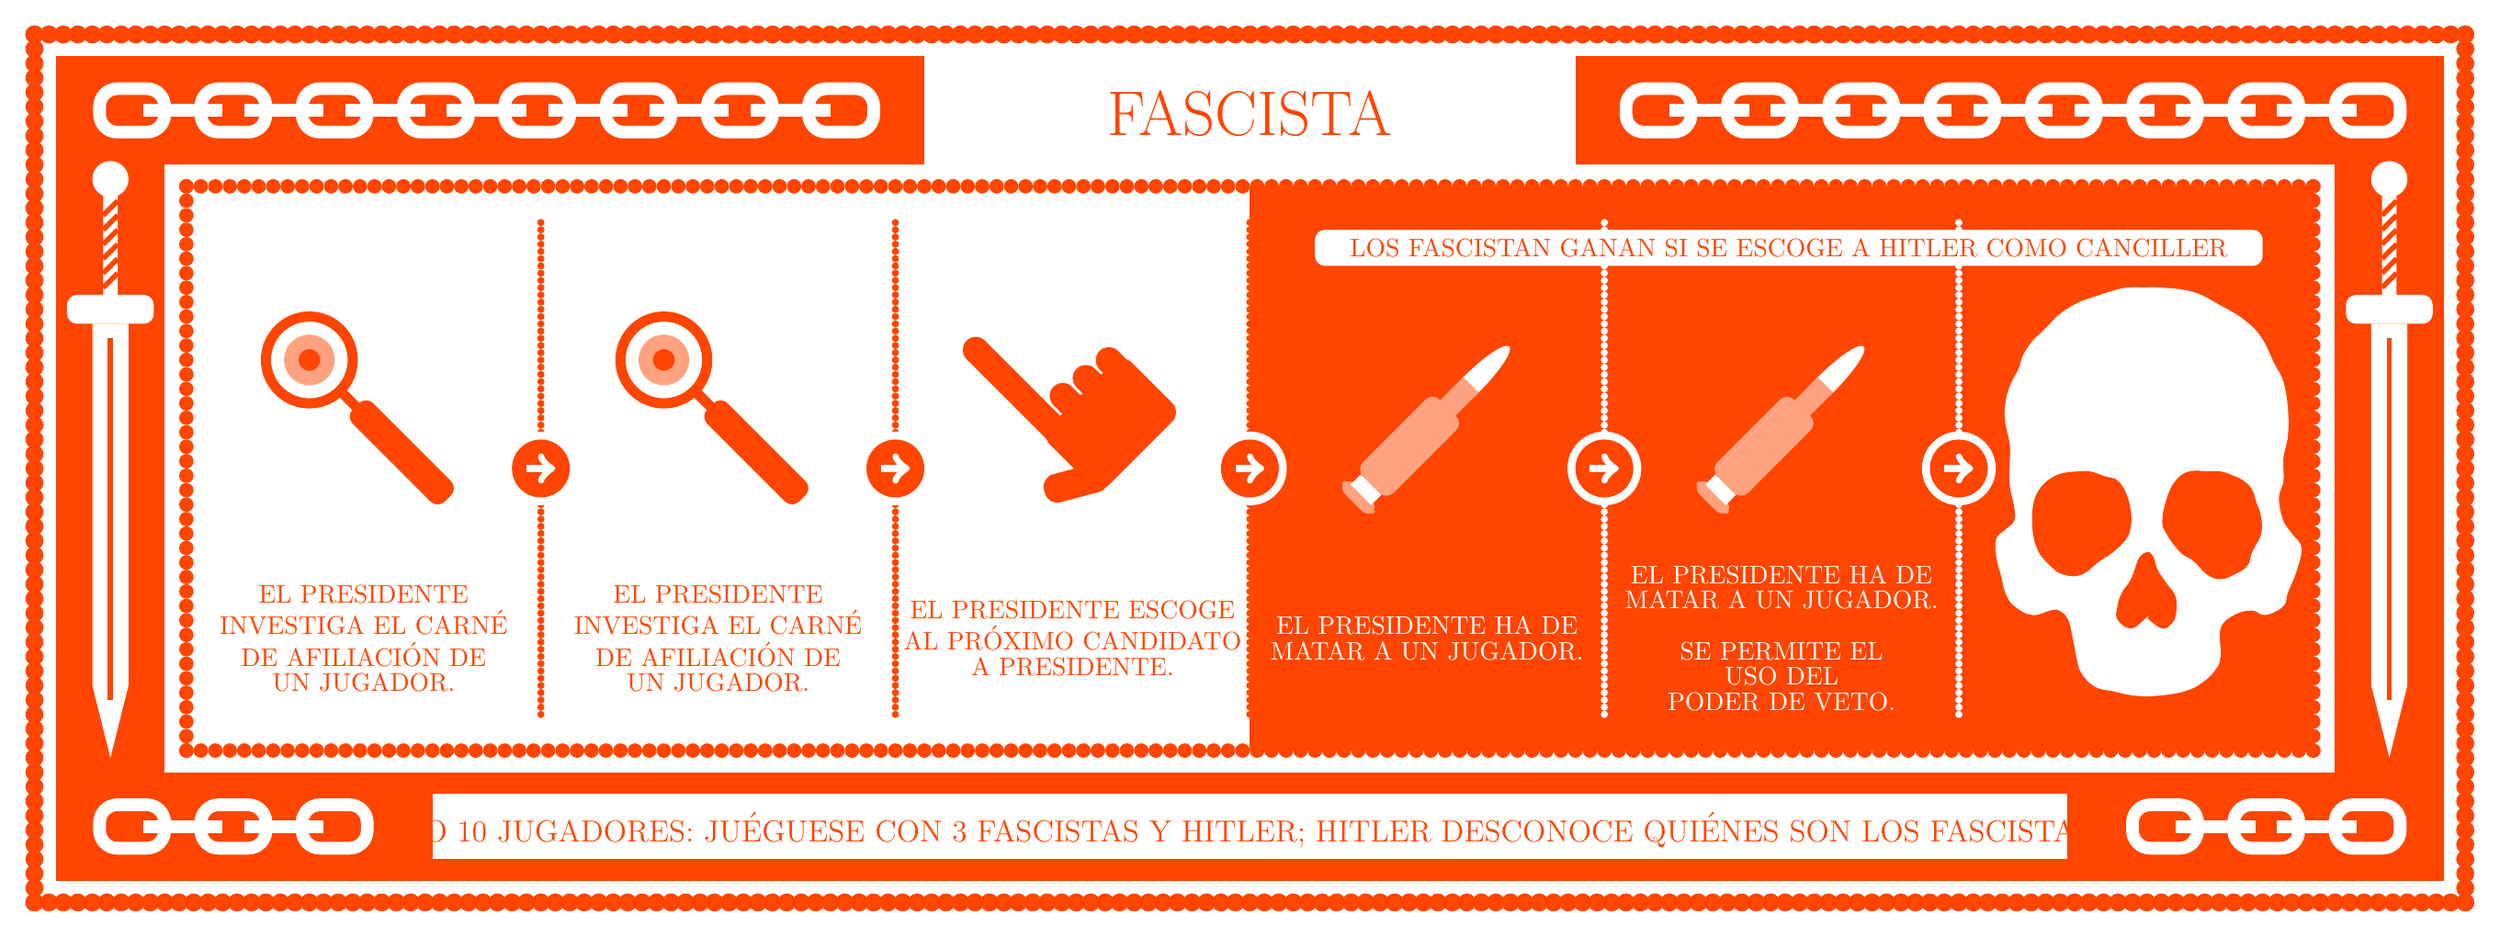
\begin{tikzpicture}		
		
		% Exterior line of points
		\foreach \y in {0,0.2,...,12}
		{
			\fill [fascist] (0,\y) circle (1.25mm);
			\fill [fascist] (33.6,\y) circle (1.25mm);
		}
		
		\foreach \x in {0, 0.2, ..., 33.6}
		{
			\fill [fascist] (\x,0) circle (1.25mm);
			\fill [fascist] (\x,12) circle (1.25mm);
		}
		
		% Interior line of points
		\foreach \y in {2.1,2.3,...,9.9}
		{
			\fill [fascist] (2.1,\y) circle (1mm);
			\fill [fascist] (31.5,\y) circle (1mm);
		}
		
		\foreach \x in {2.1, 2.3, ..., 31.5}
		{
			\fill [fascist] (\x,2.1) circle (1mm);
			\fill [fascist] (\x,9.9) circle (1mm);
		}
		
		% Central-upper text
		\node at (16.8,10.9) [fascist] {\fontsize{55}{55}\selectfont FASCISTA};
		
		% Dotted pattern for policies
		\fill [fascist] (16.8,2.1) rectangle (31.5, 9.9);
		
		% Lines of points to separate policies
		\foreach \y in {2.6,2.7,...,9.4}
		{
			\fill [fascist] (7,\y) circle (0.5mm);
			\fill [fascist] (11.9,\y) circle (0.5mm);
			\fill [fascist] (16.8,\y) circle (0.5mm);
			\fill [white] (21.7,\y) circle (0.5mm);
			\fill [white] (26.6,\y) circle (0.5mm);
		}
		
		% Arrows between policies
		\fill [white] (7,6) circle (5.1mm);
		\fill [fascist] (7,6) circle (4mm);
		\draw [line width= 3, white,->] (6.8,6)--(7.2,6);
		\fill [white] (11.9,6) circle (5.1mm);
		\fill [fascist] (11.9,6) circle (4mm);
		\draw [line width= 3, white,->] (11.7,6)--(12.1,6);
		\fill [white] (16.8,6) circle (5.1mm);
		\fill [fascist] (16.8,6) circle (4mm);
		\draw [line width= 3, white,->] (16.6,6)--(17,6);
		\fill [white] (21.7,6) circle (5.1mm);
		\fill [fascist] (21.7,6) circle (4mm);
		\draw [line width= 3, white,->] (21.5,6)--(21.9,6);
		\fill [white] (26.6,6) circle (5.1mm);
		\fill [fascist] (26.6,6) circle (4mm);
		\draw [line width= 3, white,->] (26.4,6)--(26.8,6);
		
		% Drawings over policies
		\begin{scope}[xshift=4.3 cm, yshift=7 cm]
			\draw [fascist, line width=4] (-0.5,0.5) circle (0.6);		
			\fill [fascist!50!white] (-0.5,0.5) circle (0.35);
			\fill [fascist] (-0.5,0.5) circle (0.15);
			\draw [fascist,line width=4] (-0.1,0.1)--(0.2,-0.2);
			\fill [fascist, rounded corners, rotate=-45] (0.2,0.2) rectangle (2,-0.2); 	
		\end{scope}
		\node at (4.55,3.6) [fascist] {\fontsize{10}{10}\selectfont \begin{tabular}{c}
				EL PRESIDENTE\\ INVESTIGA EL CARNÉ\\ DE AFILIACIÓN DE\\ UN JUGADOR.
		\end{tabular}};		
		
		\begin{scope}[xshift=9.2 cm, yshift=7 cm]
			\draw [fascist, line width=4] (-0.5,0.5) circle (0.6);		
			\fill [fascist!50!white] (-0.5,0.5) circle (0.35);
			\fill [fascist] (-0.5,0.5) circle (0.15);
			\draw [fascist,line width=4] (-0.1,0.1)--(0.2,-0.2);
			\fill [fascist, rounded corners, rotate=-45] (0.2,0.2) rectangle (2,-0.2); 	
		\end{scope}
		\node at (9.45,3.6) [fascist] {\fontsize{10}{10}\selectfont \begin{tabular}{c}
			EL PRESIDENTE\\ INVESTIGA EL CARNÉ\\ DE AFILIACIÓN DE\\ UN JUGADOR.
		\end{tabular}};		
	
		\begin{scope}[xshift=13.45cm, yshift=7.2cm]
			\fill [fascist, rounded corners=5, rotate=-45] (-0.80,-0.18) rectangle(1.3,0.18);
			\fill [fascist, rounded corners=5, rotate=-45] (0.5,0.22) rectangle(1.3,0.58);
			\fill [fascist, rounded corners=5, rotate=-45] (0.55,0.62) rectangle(1.3,0.98);
			\fill [fascist, rounded corners=5, rotate=-45] (0.6,1.02) rectangle(1.3,1.38);
			\fill [fascist, rounded corners=5, rotate=-45] (0.85,-0.2) rectangle(2,1.4);
			\fill [fascist, rounded corners=5, rotate=15] (0.1,-1.8) rectangle(1,-1.4);
		\end{scope}
		\node at (14.35,3.6) [fascist] {\fontsize{10}{10}\selectfont \begin{tabular}{c}
				EL PRESIDENTE ESCOGE\\ AL PRÓXIMO CANDIDATO\\ A PRESIDENTE.
		\end{tabular}};	
		
		\begin{scope}[xshift=18.3 cm, yshift=5.6 cm]
			\fill [white, rotate=-45] (0,2.2) ellipse (0.15 and 0.75);
			\fill [fascist!50!white, rounded corners, rotate=-45] (-0.3,-0.1) rectangle (0.3,0.1);
			\fill [white, rotate=-45] (-0.2,0.05) rectangle (0.2,0.25);
			\fill [fascist!50!white, rotate=-45, rounded corners] (-0.3,0.25) rectangle (0.3,1.75);
			\fill [fascist!50!white, rotate=-45] (-0.15,1.75) rectangle (0.15,2.2);
		\end{scope}
		\node at (19.25,3.6) [white] {\fontsize{10}{10}\selectfont \begin{tabular}{c}
				EL PRESIDENTE HA DE\\ MATAR A UN JUGADOR.
		\end{tabular}};
	
		\begin{scope}[xshift=23.2 cm, yshift=5.6 cm]
			\fill [white, rotate=-45] (0,2.2) ellipse (0.15 and 0.75);
			\fill [fascist!50!white, rounded corners, rotate=-45] (-0.3,-0.1) rectangle (0.3,0.1);
			\fill [white, rotate=-45] (-0.2,0.05) rectangle (0.2,0.25);
			\fill [fascist!50!white, rotate=-45, rounded corners] (-0.3,0.25) rectangle (0.3,1.75);
			\fill [fascist!50!white, rotate=-45] (-0.15,1.75) rectangle (0.15,2.2);
		\end{scope}
		\node at (24.15,3.6) [white] {\fontsize{10}{10}\selectfont \begin{tabular}{c}
				EL PRESIDENTE HA DE\\ MATAR A UN JUGADOR.\\\\SE PERMITE EL\\USO DEL\\ PODER DE VETO.
		\end{tabular}};
		
		% Fascist logo on last policy
		\begin{scope} [xshift=34cm,yshift=5.4cm,scale=0.31]
			\fill [white] plot[smooth, tension=.7] coordinates {(-15.6,10) (-16.4,10) (-17.2,9.8) (-17.8,9.6) (-18.4,9.4) (-18.8,9.2) (-19.4,8.8) (-19.8,8.4) (-20.2,8) (-20.6,7.6) (-21,7) (-21.2,6.4) (-21.6,5.6) (-21.8,4.8) (-21.8,4) (-21.6,3) (-21.6,2.2) (-21.6,1.2) (-21.4,0.2) (-21.4,-0.4) (-21.8,-0.8) (-22.2,-1.2) (-22.2,-2) (-22,-2.8) (-21.8,-3.6) (-21.4,-4.2) (-20.6,-4.6) (-19.8,-4.4) (-19.4,-4.4) (-19,-4.8) (-18.8,-5.6) (-18.6,-6.6) (-18.4,-7.2) (-17.8,-7.8) (-17,-8) (-16,-8.2) (-15,-8.2) (-13.8,-8) (-13,-7.6) (-12.4,-7) (-12.2,-6.4) (-12.2,-5.2) (-11.6,-4.6) (-10.8,-4.4) (-10.2,-4.6) (-9.4,-4.2) (-9.2,-3.6) (-8.8,-2.6) (-8.6,-1.6) (-9,-1) (-9.4,-0.4) (-9.6,0.6) (-9.4,1.4) (-9.4,2.4) (-9.2,3.4) (-9.2,4.6) (-9.4,5.8) (-9.8,6.6) (-10.4,7.8) (-11.2,8.6) (-12.2,9.2) (-13.4,9.8) (-14.8,10) (-15.6,10)};
			\fill [fascist] plot[smooth, tension=.7] coordinates {(-18.6,1.8) (-18,1.8) (-17.4,1.6) (-16.8,1.4) (-16.4,0.8) (-16.2,0) (-16.2,-0.6) (-16.4,-1.2) (-17,-1.8) (-17.6,-2.2) (-18.4,-2.8) (-19.2,-2.8) (-19.8,-2.4) (-20.4,-1.6) (-20.6,-0.4) (-20.4,0.8) (-19.6,1.6) (-18.6,1.8)};
			\fill [fascist] plot[smooth, tension=.7] coordinates {(-12.8,1.8) (-12.2,1.8) (-11.6,1.6) (-11.2,1.4) (-10.8,1) (-10.6,0.4) (-10.4,-0.2) (-10.4,-1) (-10.8,-1.8) (-11,-2.4) (-11.6,-2.8) (-12.2,-3) (-12.8,-2.8) (-13.4,-2.2) (-14,-1.8) (-14.6,-1) (-14.8,-0.4) (-14.6,0.6) (-14.2,1.4) (-13.6,1.8) (-12.8,1.8)};
			\fill [fascist] plot[smooth, tension=.7] coordinates {(-15.4,-1.8) (-15.2,-2) (-15,-2.6) (-14.6,-3.2) (-14.2,-3.8) (-14.2,-4.6) (-14.4,-5) (-14.8,-5.2) (-15.4,-4.8) (-15.4,-4.6) (-15.6,-4.8) (-16.2,-5.2) (-16.8,-4.8) (-16.8,-4.2) (-16.6,-3.6) (-16.2,-3) (-15.8,-2) (-15.4,-1.8)};
		\end{scope}
	
		% Text over last three policies
		\fill [white, rounded corners] (17.7,8.8) rectangle (30.8,9.3);
		\node at (24.25, 9.05) [fascist] {\fontsize{10}{10}\selectfont LOS FASCISTAN GANAN SI SE ESCOGE A HITLER COMO CANCILLER};
		
		
		% Orange rectangles next to text
		\fill[fascist] (0.3, 11.7) rectangle(12.3,10.2);
		\fill[fascist] (33.3, 11.7) rectangle(21.3,10.2);
		
		% White chains on orange rectangles next to text
		\foreach \x in {10.7, 9.3, ..., 1.5}
		{
			\draw [white, line width=5, rounded corners=7] (\x,11.25) rectangle (\x + 0.9,10.65);
			\draw [white, line width=5] (\x - 0.8,10.95)--(\x + 0.3,10.95);
		}
		\draw [white, line width=5, rounded corners=7] (0.9,11.25) rectangle (0.9 + 0.9,10.65);
		\foreach \x in {31.8, 30.4, ..., 22}
		{
			\draw [white, line width=5, rounded corners=7] (\x,11.25) rectangle (\x + 0.9,10.65);
			\draw [white, line width=5] (\x - 0.8,10.95)--(\x + 0.3,10.95);
		}
		\draw [white, line width=5, rounded corners=7] (22,11.25) rectangle (22 + 0.9,10.65);
		
		% Decoration swords on side of central policy area
		\fill [fascist] (0.3, 10.2) rectangle(1.8, 1.8);
		\begin{scope}[xshift=1.05cm, yshift=2cm]
			\fill [white] (0,0)--(-0.25,1)--(-0.25,6)--(0.25,6)--(0.25,1)--cycle;
			\fill [white, rounded corners] (-0.6,6) rectangle (0.6,6.4);
			\fill [white, rounded corners] (-0.1,6.2) rectangle (0.1,8);
			\fill [white] (0,8) circle (2.5mm);
			\draw [fascist, line width=2] (0,0.8)--(0,5.8);
			\foreach \y in {6.5,6.7,...,7.5}
			{
				\draw [fascist, line width=2] (-0.1,\y)--(0.1,\y +0.2);
			}
		\end{scope}				
		\fill [fascist] (31.8, 10.2) rectangle(33.3, 1.8);
		\begin{scope}[xshift=32.55cm, yshift=2cm]
			\fill [white] (0,0)--(-0.25,1)--(-0.25,6)--(0.25,6)--(0.25,1)--cycle;
			\fill [white, rounded corners] (-0.6,6) rectangle (0.6,6.4);
			\fill [white, rounded corners] (-0.1,6.2) rectangle (0.1,8);
			\fill [white] (0,8) circle (2.5mm);
			\draw [fascist, line width=2] (0,0.8)--(0,5.8);
			\foreach \y in {6.5,6.7,...,7.5}
			{
				\draw [fascist, line width=2] (-0.1,\y)--(0.1,\y +0.2);
			}
		\end{scope}
		
		
		% White chains and orange rectangles on the lower side of board.
		\fill [fascist] (0.3, 0.3) rectangle (33.3,1.8);		
		\fill [white] (5.5, 0.6) rectangle (28.1,1.5);
		\foreach \x in {2.3, 3.7, ...,5}
		{
			\draw [white, line width=5, rounded corners=7] (\x,1.35) rectangle (\x + 0.9,0.75);
			\draw [white, line width=5] (\x - 0.8,1.05)--(\x + 0.3,1.05);
		}
		\draw [white, line width=5, rounded corners=7] (0.9,1.35) rectangle (0.9 + 0.9,0.75);
		\foreach \x in {31.8, 30.4, ..., 29}
		{
			\draw [white, line width=5, rounded corners=7] (\x,1.35) rectangle (\x + 0.9,0.75);
			\draw [white, line width=5] (\x - 0.8,1.05)--(\x + 0.3,1.05);
		}
		\draw [white, line width=5, rounded corners=7] (29,1.35) rectangle (29 + 0.9,0.75);
		
		% Text on lower side of the board
		\node at (16.8, 1) [fascist] {\fontsize{13}{13}\selectfont 9 O 10 JUGADORES: JUÉGUESE CON 3 FASCISTAS Y HITLER; HITLER DESCONOCE QUIÉNES SON LOS FASCISTAS.};
		
		
	\end{tikzpicture}
\end{document}